\documentclass[17pt, orivec]{extarticle} % 12pt, 14pt, 17pt, 20pt
\usepackage{amsmath}
\usepackage{amssymb}    % for \rightsquigarrow
\usepackage{wasysym}	% for frown face
\usepackage{mathrsfs} 	% for \mathscr
\usepackage{stmaryrd}
\usepackage[most]{tcolorbox}
\usepackage{ulem}
\usepackage{tikz-cd}		% commutative diagrams
\usepackage{tikz}
\usepackage{amsthm}
\usepackage{enumitem}	% for \itemize custom labels
\usepackage{turnstile}	% longer turnstiles
\usepackage[sf,bf,big,raggedright,compact]{titlesec}	% change section color to blue
% \usepackage[backend=biber,bibstyle=authoryear,citestyle=../authoryearbrack]{biblatex}
% \bibliography{../AGI-book}

\newtheorem{theorem}{Theorem}

\ifdefined\chinchin
	\newcommand{\cc}[2]{#1}
	\usepackage[CJKspace]{xeCJK}
	%\setCJKmainfont[BoldFont=SimHei,ItalicFont=AR PL KaitiM GB]{Alibaba PuHuiTi}
	\setCJKmainfont[BoldFont=Alibaba-PuHuiTi-Regular.ttf, ItalicFont=gkai00mp.ttf]{Alibaba-PuHuiTi-Light.ttf}
	% \setmainfont[ItalicFont=Latin Modern Roman Slanted]{Alibaba Sans:style=Light}
\else
	\newcommand{\cc}[2]{#2}
	% \setmainfont[ItalicFont=Latin Modern Roman Slanted]{Alibaba Sans:style=Light}
	%\renewcommand{\baselinestretch}{0.8} 
\fi

%\ifdefined\chinchin
%\newcommand{\cc}[2]{#1}
%\usepackage[CJKspace]{xeCJK}
%\setCJKmainfont[BoldFont=SimHei,ItalicFont=AR PL KaitiM GB]{SimSun}
%\else
%\newcommand{\cc}[2]{#2}
%\fi

\setlength{\headheight}{0cm}
\setlength{\hoffset}{0cm}
\setlength{\topmargin}{-2cm}
\setlength{\oddsidemargin}{-2cm}
\setlength{\evensidemargin}{-2cm}
\setlength{\textwidth}{20cm}
\setlength{\textheight}{26cm}
\setlength{\headsep}{0cm}
\setlength{\topskip}{0cm}
\setlength{\footskip}{0.9cm}  % between bottom of page and page number
\setlength{\floatsep}{0cm}
\setlength{\textfloatsep}{0.6cm}
\setlength{\intextsep}{0.5cm}
\setlength{\parindent}{0em}   % em = width of capital M

% Fix spilling of titles in bibliography:
%\DeclareFieldFormat*{title}{#1}
%
%\DeclareFieldFormat*{titlecase}{%
%    \ifdef{\currentfield}
%      {\ifcurrentfield{title}
%         {\usefield{\uline}{\currentfield}}%
%         {#1}}
%      {#1}}

\setcounter{secnumdepth}{2}		% no section numbers

\titleformat{\section}[hang]{\bfseries\Large\color{blue}}{\thesection \hspace{20pt}}{0pt}{}
\titleformat{\subsection}[hang]{\bfseries\large\color{blue}}{\thesubsection \hspace{10pt}}{0pt}{}
\titleformat{\subsubsection}[hang]{\bfseries\color{blue}}{}{0pt}{}

\itemsep0em
\setlist[itemize]{noitemsep, topsep=-5pt, partopsep=-5pt}
\renewcommand{\labelitemi}{$\textbullet$}

\let\varzero\emptyset
\let\emptyset\varnothing		% round empty set 
\newcommand{\vect}[1]{\boldsymbol{#1}}
\newcommand{\book}[1]{$\NewSym[0.4]{../book-icon.png} \quad$ \parbox{0.9\textwidth}{\footnotesize #1}}
\newcommand{\code}[1]{{\footnotesize{\ttfamily #1}}}
\newcommand{\tab}{\hspace*{2cm}}
\newcommand{\powerset}{\raisebox{.15\baselineskip}{\Large\ensuremath{\wp}}}
\newcommand{\Chi}{\raisebox{2.5pt}{$\chi$}}
\newcommand*\KB{\vcenter{\hbox{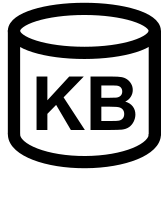
\includegraphics{../KB-symbol.png}}}}
\newcommand*\NewSym[2][0.5]{\vcenter{\hbox{\includegraphics[scale=#1]{#2}}}}
\newcommand*\sigmoid{\vcenter{\hbox{
\includegraphics{../sigmoid3.png}}}}
\newcommand{\smbox}[1]{\boxed{\footnotesize{\mbox{#1}}}}

\newcommand{\tikzmark}[1]{\tikz[overlay,remember picture] \node (#1) {};}

\newcommand{\Dfrac}[2]{%
\ooalign{%
      $\genfrac{}{}{2.9pt}0{\hphantom{#1}}{\hphantom{#2}}$\cr%
      $\color{white}\genfrac{}{}{1.5pt}0{\hphantom{#1}}{\hphantom{#2}}$\cr%
      $\color{white}\genfrac{}{}{1pt}0{\color{black}#1}{\color{black}#2}$}}

% \renewcommand{\thefootnote}{\fnsymbol{footnote}}
\usepackage{perpage}
\MakePerPage{footnote}
\renewcommand{\thefootnote}{\ifcase\value{footnote}\or{*}
	\or{$\dagger$}\or{**}\or{$\ddagger$}\fi}
\interfootnotelinepenalty=10000

\setlength{\parindent}{0pt}
\setlength{\parskip}{1.8ex plus0.8ex minus0.8ex}

% Note: for best effect, use font size 12pt in YKY-preamble
% \usepackage[no-math]{fontspec}
% \setmainfont[BoldFont=Alibaba_Sans_Regular.otf,ItalicFont=Alibaba_Sans_Light_Italic.otf]{Alibaba_Sans_Light.otf}

%\usepackage[backend=biber]{biblatex}
%\bibliography{../AGI-book}

\usepackage{wrapfig}			% for Henry George pic

\usepackage[active,tightpage]{preview}		% for continuous page(s)
\renewcommand{\PreviewBorder}{0.5cm}
\renewcommand{\thempfootnote}{\arabic{mpfootnote}}

\usepackage[absolute,overlay]{textpos}		% for page number on upper left corner

\usepackage{color}
% \usepackage{mathtools}
\usepackage[hyperfootnotes=false]{hyperref}

% \usepackage[backend=biber,style=numeric]{biblatex}
% \bibliography{../AGI-book}
% \renewcommand*{\bibfont}{\footnotesize}

\usetikzlibrary{shapes}
% \usepackage[export]{adjustbox}	% ??
\usepackage{verbatim} % for comments
% \usepackage{newtxtext,newtxmath}	% Times New Roman font

% \titleformat{\subsection}[hang]{\bfseries\large\color{blue}}{}{0pt}{}
% \numberwithin{equation}{subsection}

\newcommand{\underdash}[1]{%
	\tikz[baseline=(toUnderline.base)]{
		\node[inner sep=1pt,outer sep=10pt] (toUnderline) {#1};
		\draw[dashed] ([yshift=-0pt]toUnderline.south west) -- ([yshift=-0pt]toUnderline.south east);
	}%
}%

\newcommand\reduline{\bgroup\markoverwith{\textcolor{red}{\rule[-0.5ex]{2pt}{0.4pt}}}\ULon}

%\DeclareSymbolFont{symbolsC}{U}{txsyc}{m}{n}
%\DeclareMathSymbol{\strictif}{\mathrel}{symbolsC}{74}
%\DeclareSymbolFont{AMSb}{U}{msb}{m}{n}
%\DeclareSymbolFontAlphabet{\mathbb}{AMSb}
%\setmathfont{lmroman17-regular.otf}
\DeclareMathOperator*{\argmin}{arg\,min}
\DeclareMathOperator*{\argmax}{arg\,max}

% \usepackage[most]{tcolorbox}
%\tcbset{on line,
%	boxsep=4pt, left=0pt,right=0pt,top=0pt,bottom=0pt,
%	colframe=red,colback=pink,
%	highlight math style={enhanced}
%}
%\newcommand{\atom}{\vcenter{\hbox{\tcbox{....}}}}

\let\oldtextbf\textbf
\renewcommand{\textbf}[1]{\textcolor{blue}{\oldtextbf{#1}}}

\newcommand{\logic}[1]{{\color{violet}{\textit{#1}}}}
\newcommand{\underconst}{
\includegraphics[scale=0.5]{../2020/UnderConst.png}}
\newcommand{\KBsymbol}{\vcenter{\hbox{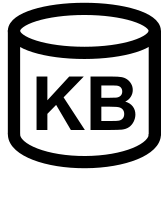
\includegraphics[scale=1]{../KB-symbol.png}}}}
\newcommand{\token}{\vcenter{\hbox{\includegraphics[scale=1]{token.png}}}}
\newcommand{\proposition}{\vcenter{\hbox{\includegraphics[scale=0.8]{proposition.png}}}}

\newtcolorbox{mybox}{
	enhanced,
	boxrule=1pt,
	colback=yellow!40!white,
	sharp corners
}

\begin{document}

\begin{preview}

\title{\vspace{-1cm} \bfseries\color{blue}{\huge \cc{Georgism 应用到 全民医保}{Henry George applied to Universal Health Care}}}

% \author{YKY} % Your name
% \date{\vspace{-2.5cm}}
% \date{\tiny\today}
\date{\vspace{-1.5cm} \small \today}

\maketitle

%\vspace{-3.5cm}
%\hfill{\tiny\today}
%\vspace*{1.5cm}

\setcounter{section}{-1}
\newcounter{mypage}
\setcounter{mypage}{0}

% (1) Circled page number on upper left corner
%\begin{textblock*}{5cm}(2.1cm,2.3cm) % {block width} (coords)
%{\color{red}{\large \textcircled{\small \themypage}}}
%\addtocounter{mypage}{1}
%\end{textblock*}

\begin{minipage}{\textwidth}
\setlength{\parskip}{0pt}

\section{Henry George 关于地产霸权的思想}

``\textbf{Affordable housing}'' 这个术语 可以被翻译成「可负担住房」,但不纯粹是「廉价住房」那么简单。 它更接近于 习近平 所说的「房是用来住,不是用来炒」的意思,简称「\textbf{房住不炒}」。\\

其实 这个问题 很可能 已经在差不多一个半世纪以前 被美国经济学家 Henry George 解决了。 他提出的方案是征收 \textbf{地税} (land tax) 来解决土地未被有效运用的问题。 土地税 可以阻止人们垄断土地 作为 “rent-seeking” 的弊端,也就是阻止 炒卖地产。 但这个想法一直没有被执政者 实施过,因为人们根深蒂固地认为 房地产 是经济的重要部分。\\

\begin{wrapfigure}[9]{l}{3cm}		% first number = # of lines of narrow text
	\label{wrap-fig:1}
	\vspace{-0.5cm}
	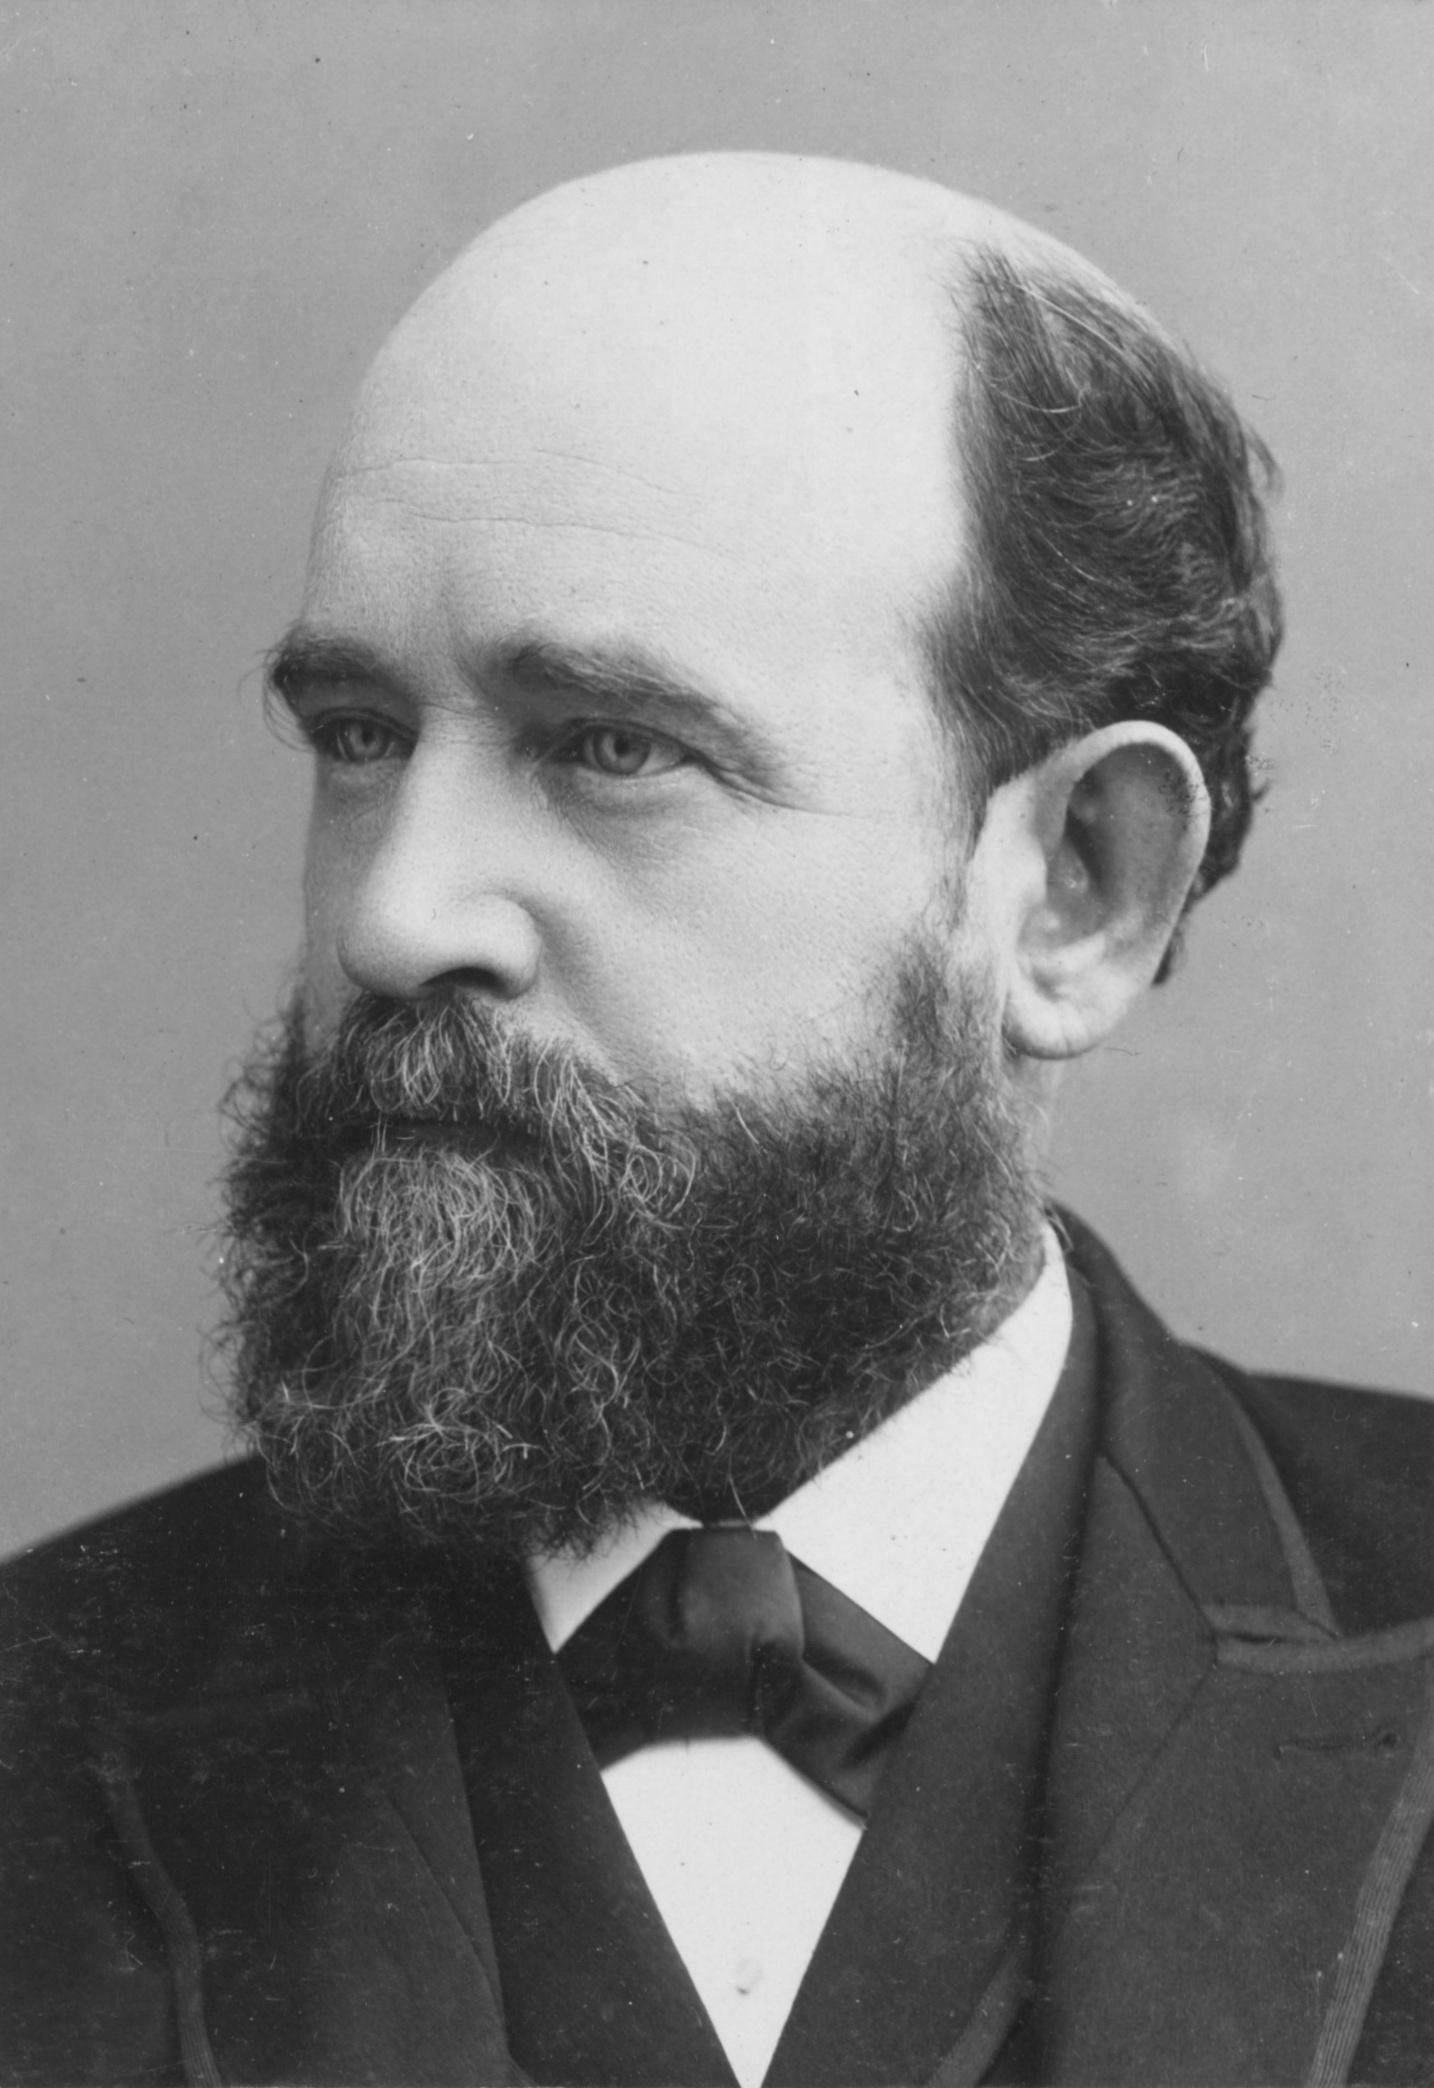
\includegraphics[width=3cm]{Henry-George.jpg}
\end{wrapfigure}
\textit{Henry George (1839-1897) 是他那时代 美国最有名的人之一。 他曾经参选 纽约 市长,但不幸在选举前 中风病逝。他的「粉丝」包括 孙中山、爱因斯坦、Tolstoy、马克$\cdot$吐温、George Bernard Shaw、甚至 马克思、和当代 自由主义经济学家 Milton Friedman、新凯因斯学派的 Joseph Stiglitz 等。 他和他的追随者有时被称为 “圣徒”,他自己有时也用神学的语言谈论经济学。 有人说,出于妒忌,同时代的经济学家 排斥和试图掩盖他的学说。 和马克思提出的共产主义不同之处是,George 认为 {\color{blue}\ 自由竞争} 是自然而合理的。 也可以说 Georgism 是一种社会主义,虽然他不喜欢 socialism 这个用语,但我纯粹用它表示不同于 共产主义极端 的任何较温和的左派思想。} \\

\section{将 ``Georgism'' 应用到 全民医保}

在数学上,有所谓 ``functor'' 的概念,意思是 将一个问题的解决方案,经过抽象以后,应用到另一个不同的问题上,``changing what needs to be changed'':
\begin{equation}
\begin{tikzcd}[column sep=2.5cm, row sep=2cm]
\mbox{问题 1} \arrow[r, "functor"]
\arrow[r, to path={ -- ([yshift=4ex]\tikztostart.north) -| (\tikztotarget)},
rounded corners=12pt, dashed, red]
\ar[phantom]{r}[yshift=8ex]{\footnotesize{\mbox{\color{red}将左边的解决方案,经过抽象后,应用到右边}}}
% \arrow[r, dashed, bend left=90, "\footnotesize{\mbox{将左边的解决方案,经过抽象后,应用到右边}}"]
& \mbox{问题 2}
\end{tikzcd}
\nonumber
\end{equation}
而我一直在思考的问题,就是如何将 George 对土地问题的解决方案 ``func'' 到 全民医保的问题上。 \\

George 的地税思想,其抽象本质就是: 由于 土地 是 \textbf{稀缺资源},而且它是 人类 \textbf{生命必需} 的资源,所以对它进行 征税 是合理的。 古典经济学的中心思想是 自由市场的 「看不见的手」,而 征税是属于自由市场之外的 ``externality''.  这一点在「资源经济学」或「环境经济学」里得到了肯定。 举例来说: 拥有河流上游的人不应该随便污染下游的水,因为水是 \textbf{稀缺而且生命必需} 的资源,所以它可以 \textbf{例外于} 自由市场的供求定律。\\

那么根据这个看法,将 Georgism 转换到全民医保的方法,似乎就是:
\begin{eqnarray}
	\fcolorbox{black}{yellow}{\mbox{土地}} & \longrightarrow \mbox{征税} \nonumber \\
	\fcolorbox{black}{yellow}{\mbox{医疗资源}} & \longrightarrow \mbox{征税} \nonumber
\end{eqnarray}
所不同的是,土地是一种 passive 的资源,但「医疗」是一种 active, 复杂 而 dynamic 的资源,它本身是经济活动的成果。 这就是 ``what needs to be changed'' 的部分。 这个做法的好处是它保留了 医疗领域的 \textbf{自由竞争},而这是 医疗技术 进步的必要条件。\\

我暂时仍未弄清细节,但有一点好像违反直观: 对医疗资源 征税,岂不是减弱了人们 投资医疗领域的意欲? 然而,医疗行业 的一个难题 明显就是(公立医院的)医护人员 over-worked and underpaid.  那这个有待提出的税收,有没有可能 反直观地 解决医护人手不足的问题?

\end{minipage}
\end{preview}

\begin{comment}
\begin{preview}
\begin{textblock*}{5cm}(2.1cm,2.3cm) % {block width} (coords)
	{\color{red}{\large \textcircled{\small \themypage}}}
	\addtocounter{mypage}{1}
\end{textblock*}

\begin{minipage}{\textwidth}
	\setlength{\parskip}{0.4\baselineskip}

\section{This}

\begin{itemize}
	\item Here
\end{itemize}

\end{minipage}
\end{preview}

\begin{preview}
\begin{textblock*}{5cm}(2.1cm,2.3cm) % {block width} (coords)
{\color{red}{\large \textcircled{\small \themypage}}}
\addtocounter{mypage}{1}
\end{textblock*}

\begin{minipage}{\textwidth}
\setlength{\parskip}{0.4\baselineskip}

\section{This}

\begin{itemize}
	\item Here
\end{itemize}

\end{minipage}
\end{preview}

\begin{preview}
\begin{textblock*}{5cm}(2.1cm,2.3cm) % {block width} (coords)
	{\color{red}{\large \textcircled{\small \themypage}}}
	\addtocounter{mypage}{1}
\end{textblock*}

\begin{minipage}{\textwidth}
	\setlength{\parskip}{0.4\baselineskip}

\section{This}

\begin{itemize}
	\item Here
\end{itemize}

\end{minipage}
\end{preview}

\end{comment}

\end{document}
